\section{Versuchsaufbau und Durchführung}
\label{sec:Durchführung}
Der Versuchsaufbau wird schematisch in der Abbildung \ref{fig:versuchsaufbau} dargestellt. Da die $\alpha$-Teilchen eine geringe Reichweite($\SI{10}{\centi\meter}$) in Luft haben, wird der Versuch in Vakuum durchgeführt, um die Wechselwirkung mit den Stoßpartnern(Luftmolekülen), an die die $\alpha$-Teilchen ihre kinetische Energie sukzessive abgeben, zu verhindern. Die $\alpha$-Teilchen verlieren bereits in Luft rasch an Intensität, da sie mehr Energie an ihre Umgebung abgeben. Als Quelle dient ein $^{241}$Am-Präparat, das mit einer Halbwertszeit von $420$ Jahren zu Neptunium zerfällt.
\begin{figure}[h!]
	\centering
	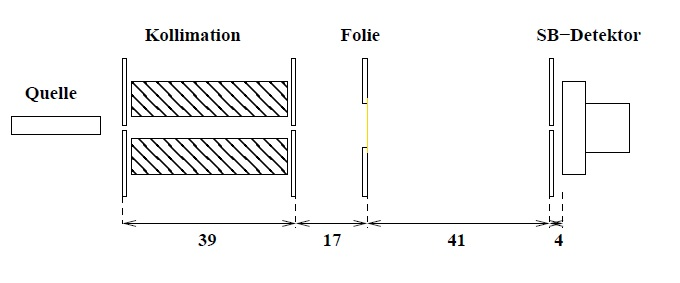
\includegraphics[width=0.9\linewidth]{../Versuchsaufbau}
	\caption{Schematischer Aufbau des Versuches, \cite[2]{anleitungV16}.}
	\label{fig:versuchsaufbau}
\end{figure}
Die Strahlen aus der Quelle werden mithilfe von zwei $\SI{2}{\milli\meter}$ Schlitzblenden kollimiert und werden durch die Blenden gebündelt. Der Strahl trifft anschließend senkrecht auf die Goldfolie, wo dann die Wechselwirkung mit Materie stattfindet. Die gestreuten $\alpha$-Teilchen werden in Abhängigkeit des Streuwinkels von einem Halbleiter-Detektor, also einen Surface-Barrier-Detektor detektiert. Bei diesem Detektor handelt es schließlich um eine in Sperrrichtung betriebene Diode, wo die einfallenden $\alpha$-Teilchen Elektronen-Loch-Paare erzeugen, die zur Elektrode beschleunigt werden. Der aufgenommene Impuls wird durch einen Multiplier verstärkt und ist proportional zur Energie des Teilchens. Außerdem sind noch ein Oszilloskop für die Energieverlustmessung und ein Zähler für die Streuquerschnittmessung vorhanden.

Zuerst wird die Streukammer mit einer Vakuumpumpe evakuiert. Die Sperrspannung des Surface-Barrier-Detektors wird auf $\SI{12}{\volt}$ eingestellt. Der Detektor wird justiert, damit die $\alpha$-Teilchen einen geraden Durchtritt bekommen können. Anschließend wird eine Energieverlustmessung der Foliendicke durchgeführt. Dazu wird die Pulshöhe der Detektorpulse in Abhängigkeit von verschiedenen Kammerdrücken gemessen. Dieser Messvorgang wird zunächst mit und anschließend ohne eingesetzter Folie durchgeführt. Mithilfe von einem Feindrosselventil wird der Kammerdruck langsam erhöht. Die Funktion "Nachleuchten" wird am Ozilloskop eingestellt um die mittleren Pulshöhen zu ermitteln und an dem werden die Pulshöhe abgelesen. Im weiteren Verlauf des Versuches sollte der differentielle Streuquerschnitt für eine dünne Goldfolie untersucht werden. Hierfür wird die Zählrate in Abhängigkeit des Streuwinkels gemessen. Für diese Messung werden verschiedene Winkel benötigt. Da der der $\alpha$-Zerfall poissonverteilt ist, wird versucht den Fehler möglichst klein zu halten. Der statistische Fehler dieser Messung für die Zählrate beträgt $\sqrt{I}$. Für die Messung der Mehrfachstreuung wird der Streuquerschnitt mithilfe von einer anderen Goldfolie mit einer anderen Dicke bei einem festen Winkel von $15 ^circ$ gemessen.

